\documentclass{article}
\usepackage{graphicx}
\graphicspath{ {./images/} }
\usepackage[export]{adjustbox}
\usepackage{amsmath}
\usepackage{polynom}


\title{11. Polinomu dalīšana}
\author{Gunārs Ābeltiņš}
\date{2022-05-19}

\begin{document}

\maketitle

\section*{1. Uzdevums}
Izdaliet polinomu x6-x4+x3-2x2+5x-9 ar polinomu x3-3x+4, iegūstot dalījumu un atlikumu. Rezultātu pārbaudiet ar WolframAlpha.

\polylongdiv{x^6-x^4+x^3-2x^2+5x-9}{x^3-3x+4}
\begin{equation*}
    \frac{x^6-x^4+x^3-2x^2+5x-9}{x^3-3x+4} = x^3 + 2x - 3 + \frac{4x^2-12x+3}{x^3-3x+4}
\end{equation*}
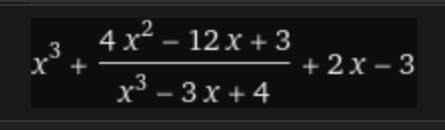
\includegraphics[width=0.3\textwidth, center]{1}

\section*{2. Uzdevums}
Izdaliet polinomu 6x4-5x3-4x2+23x-27 ar polinomu 2x2-3x+4, iegūstot dalījumu un atlikumu. Rezultātu pārbaudiet ar WolframAlpha.

\polylongdiv{6x^4-5x^3-4x^2+23x-27}{2x^2-3x+4}
\begin{equation*}
    \frac{6x^4-5x^3-4x^2+23x-27}{2x^2-3x+4} = 3x^2 + 2x - 5 + \frac{-7}{2x^2-3x+4}
\end{equation*}
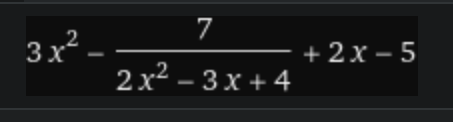
\includegraphics[width=0.3\textwidth, center]{2}

\section*{3. Uzdevums}
Uzbūvējiet 5.pakāpes polinomu, kam nav divu vienādu koeficientu, un kas, dalot to ar x2+x+1, dod atlikumā x+1.

\polylongdiv{x^5+3x^4+6x^3+9x^2+8x+5}{x^2+x+1}
\begin{equation*}
    \frac{x^5+3x^4+6x^3+9x^2+8x+5}{x^2+x+1} = x^3 + 2x^2 + 3x + 4 + \frac{x+1}{x^2+x+1}
\end{equation*}

\end{document}